\documentclass[svgnames,dvipsnames,aspectratio=169]{beamer}
\usepackage[english]{babel}
\usepackage[utf8x]{inputenc}
\usepackage[T1]{fontenc}
\usepackage{lmodern}
\usepackage{amsmath}
\usepackage{amssymb}
\usepackage{multicol}
\usepackage{multirow}
\usepackage{array}
\usepackage[absolute,overlay]{textpos}
\usepackage{xcolor,pgf,colortbl}
\usepackage{appendixnumberbeamer}
\usepackage{tikz}
\usetikzlibrary{positioning,calc}
\usetikzlibrary{arrows,shapes}
\usepackage[percent]{overpic}
\usepackage{color}
\usepackage{transparent}
\usepackage{graphicx} % Allows including images
\usepackage{etoolbox}
\usepackage{forloop}
\usepackage{calc}
\usepackage{algorithmic}
\usepackage{tabularx}
\usepackage{pgffor}
\usepackage{xspace}
\usepackage{xstring}
\usepackage{grffile}

\DeclareGraphicsExtensions{%
  .pdf,.PDF,%
  .png,.PNG,%
  .jpg,.mps,.jpeg,.jbig2,.jb2,.JPG,.JPEG,.JBIG2,.JB2}

\renewcommand*\sfdefault{ugq}

\mode<presentation> {
  \usetheme{Boadilla}
  \usecolortheme{default}
  \setbeamertemplate{navigation symbols}{} % To remove the navigation symbols from the bottom of all slides uncomment this line
}



\definecolor{Gray}{gray}{0.85}
\newcolumntype{a}{>{\columncolor{Gray}}c}

% % % % % % % % % % % % % % % % % % % % %
% Document wide variables and definitions
% Text variables
\newcommand{\Pt}{\ensuremath{\boldsymbol{p_{\text{T}}}}\xspace}
\newcommand{\pt}{\Pt}
\newcommand{\Nsigma}{\ensuremath{\boldsymbol{N-\sigma}}\xspace}
\newcommand{\Nsig}{\Nsigma}
\newcommand{\nsigma}{\Nsigma}
\newcommand{\tztof}{\ensuremath{\boldsymbol{t_{0, TOF}}}\xspace}
\newcommand{\circa}[1]{\ensuremath{\boldsymbol{\sim #1}}\xspace}
\newcommand{\fd}{\ensuremath{\boldsymbol{\longrightarrow}}\ }
\newcommand{\chitwo}{\ensuremath{\boldsymbol{\chi^{2}}}\xspace}
\newcommand{\deltax}{\ensuremath{\boldsymbol{\delta_{\rm x}}}\xspace}
\newcommand{\boldeta}{\ensuremath{\boldsymbol{\eta}}\xspace}
\newcommand{\boldphi}{\ensuremath{\boldsymbol{\phi}}\xspace}
\newcommand{\mevc}{\ensuremath{\boldsymbol{{\rm MeV}/c}}\xspace}

% % % % % % % % % % % % % % % % % % % % %



%----------------------------------------------------------------------------------------
% TITLE PAGE
%----------------------------------------------------------------------------------------

\makeatletter
\setbeamertemplate{title page}
{
  \vbox{}
  \vfill
  \begin{centering}
    \setbeamercolor{title}{bg=white,fg=structure}
    \setbeamercolor{author}{bg=white,fg=structure}
    \vbox to 1.\textheight{
      \vfill
      \centering
      \hspace*{-.4cm}
      \resizebox{\paperwidth}{!}{
        {\transparent{.6}%
            \begin{beamercolorbox}[sep=8pt]{title}
              \transparent{1.}%
              \usebeamerfont{title}\inserttitle
              \vskip.5cm\par
              \usebeamerfont{author}\insertauthor
              \vskip.2cm\par
              \begin{columns}
                \column{.7\textwidth}
                \usebeamerfont{institute}\insertinstitute
                %\vskip.5cm\par
                %\hfill
                %\par
                \column{.1\textwidth}
                \column{.1\textwidth}
                {\usebeamercolor[fg]{titlegraphic}\inserttitlegraphic\par}
              \end{columns}
              \ifx\insertsubtitle\@empty%
              \else%
                \vskip0.25em%
                {\usebeamerfont{subtitle}\usebeamercolor[fg]{subtitle}\insertsubtitle\par}%
              \fi%
              \hfill\hfill
              %\vskip1em\par
              \vskip-.2cm\par
              %\usebeamerfont{date}\insertdate
              \vskip-.2cm\par
            \end{beamercolorbox}
          }
      }
      \hfill
    }
  \end{centering}
  \vfill
}


\begin{document}

\title[TOF QA]{ {\Huge TOF QA report} } % The short title appears at the bottom of every slide, the full title is only on the title page
\subtitle{\Large Data period -- {{ periodname }} {{ passname }} } % The short title appears at the bottom of every slide, the full title is only on the title page

\author[ {{ presenter }}]{
  {{ authors }}\\
  on behalf of the TOF group
} % Your name



\titlegraphic{
  
\includegraphics[width = \textwidth, keepaspectratio=true]{images/4_Color_Logo_CB.png}
}
\institute[ {{ presenterinstitute }} ] % Your institution as it will appear on the bottom of every slide, may be shorthand to save space
{
  {
      \tiny
      {{ institutes }}
    }
  \\
  \medskip

  {
    \large
    QA meeting -- \today
  }

  \medskip

}


{
  \centering
  \usebackgroundtemplate{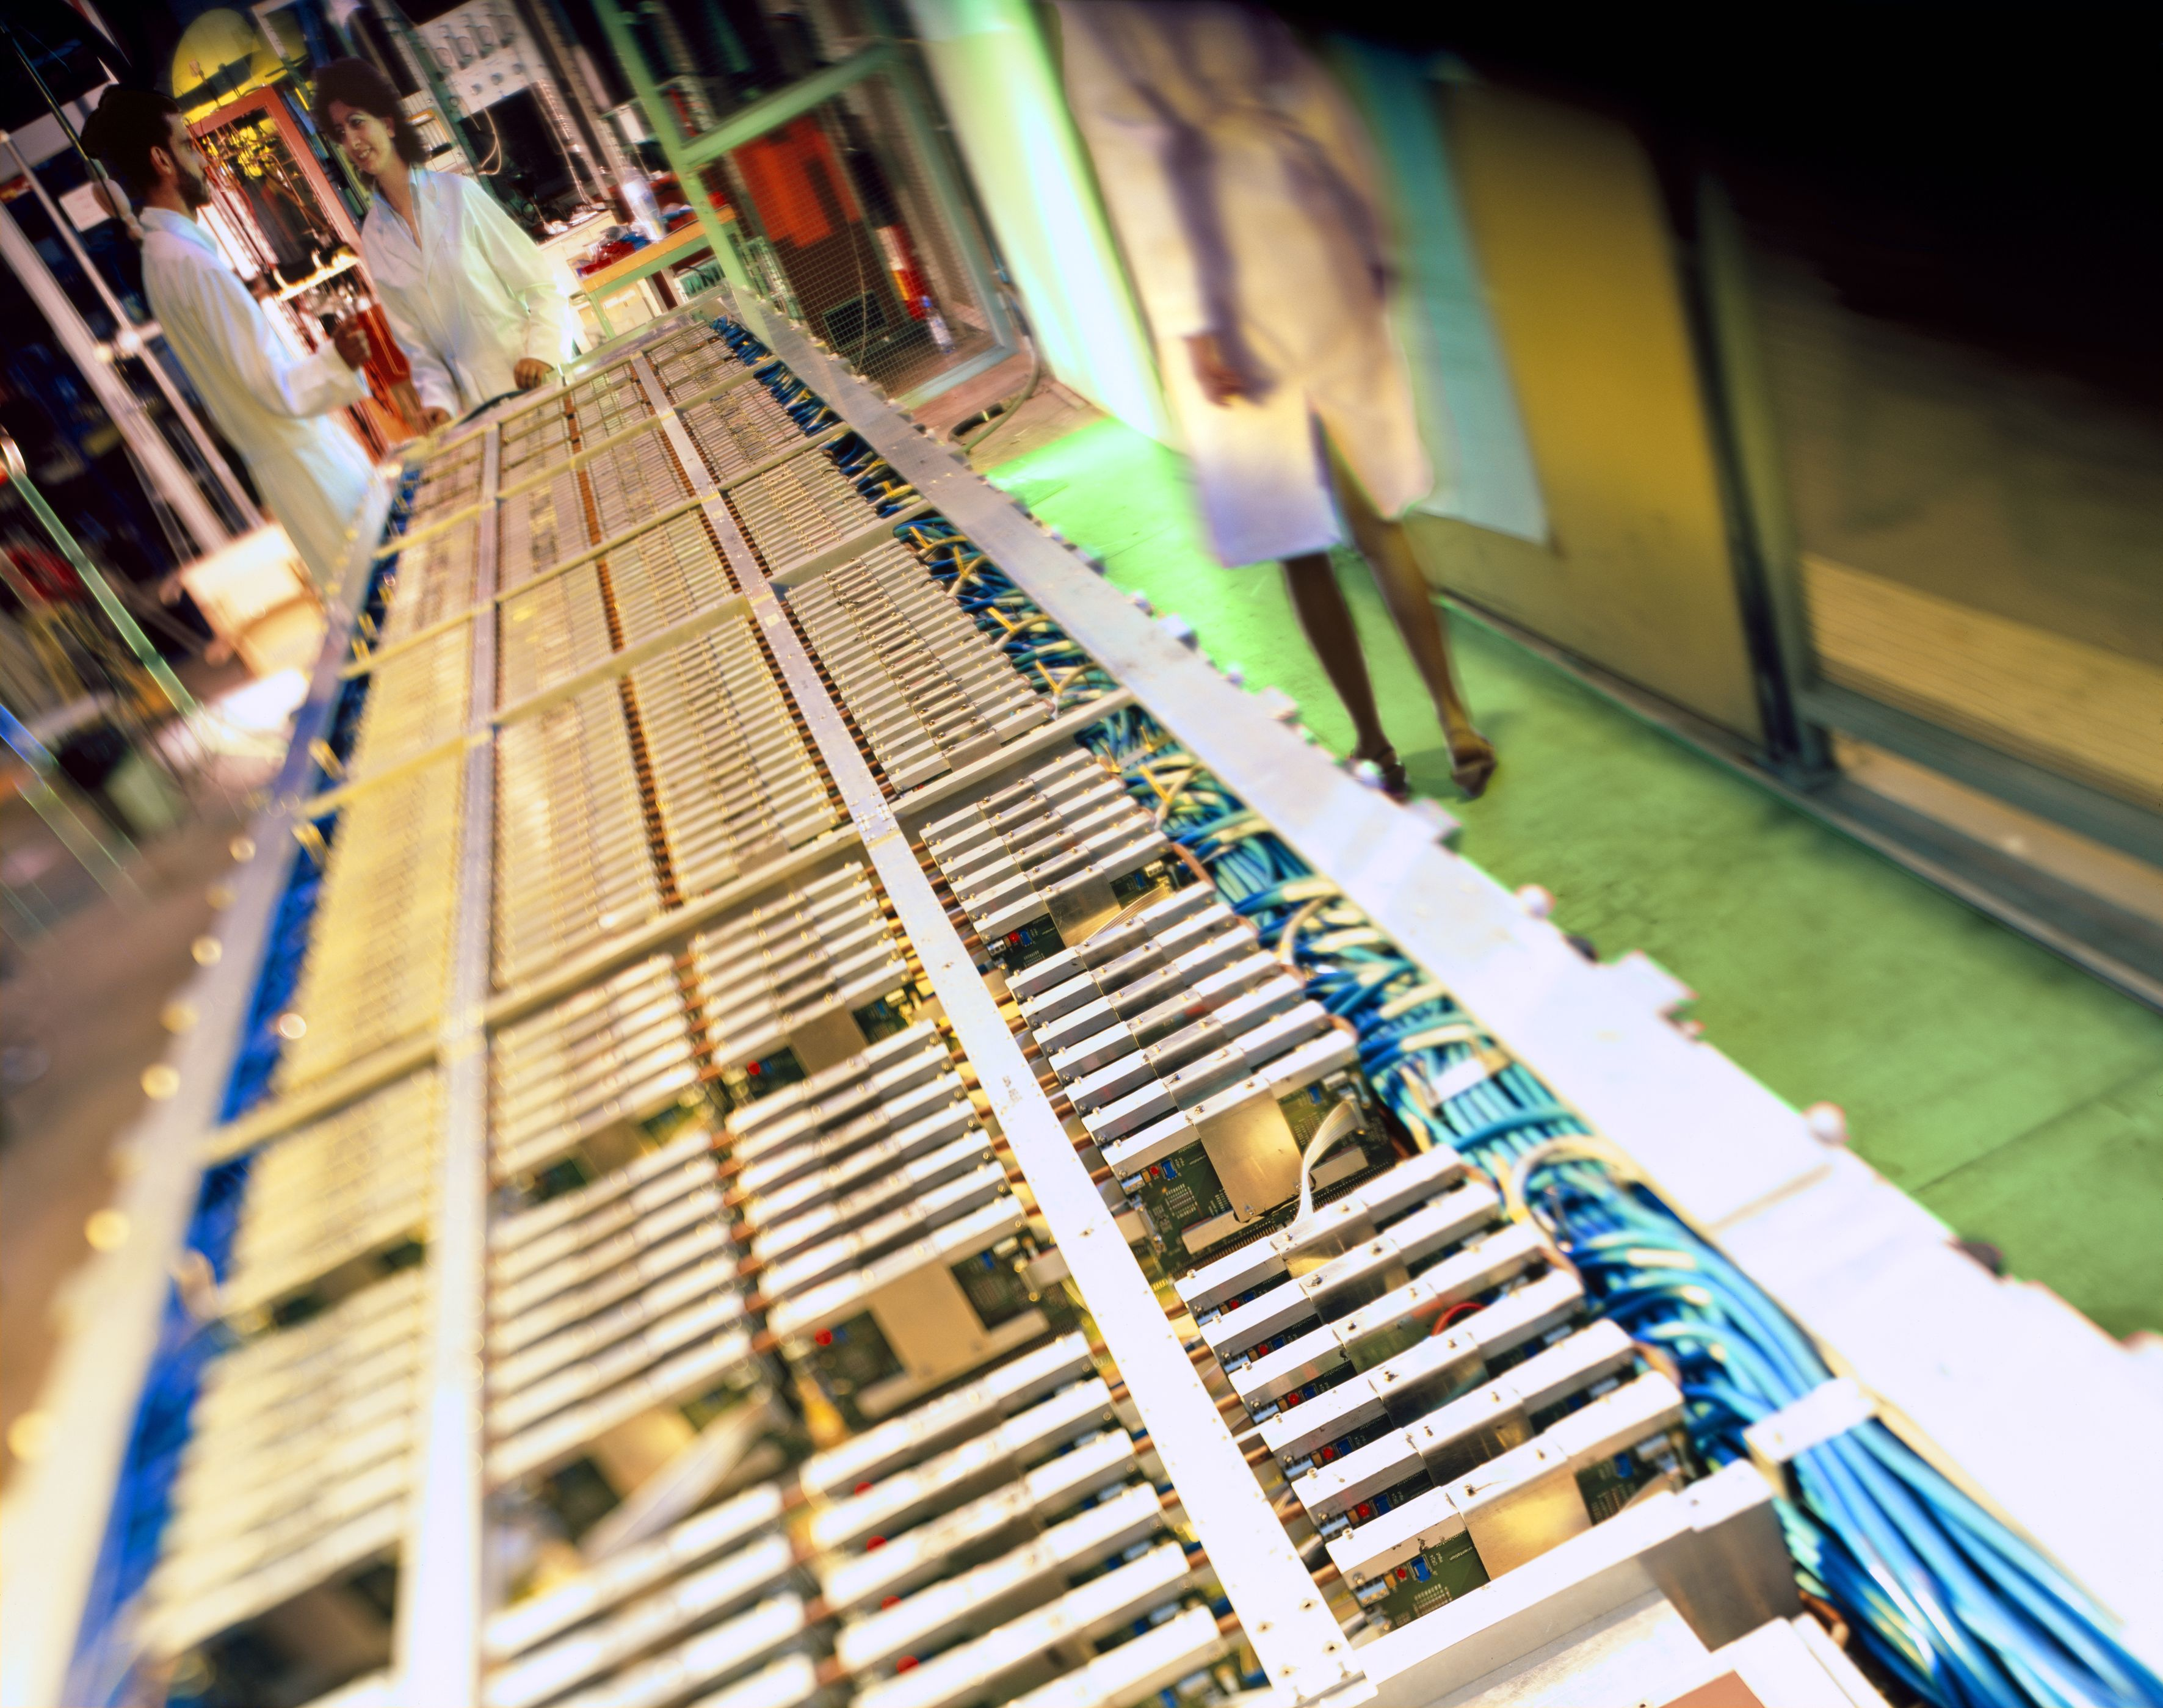
\includegraphics[trim = 0 0 0 300, clip,width=\paperwidth,keepaspectratio]{images/tof-2006-011}}
  \begin{frame}
    \maketitle
  \end{frame}
}

%\begin{frame}{Matching efficiency {{ titletag }}}
  \includegraphics[width=\textwidth]{{ '{' }}{{ imagepath }}mDeltaXEtaUNCONS}\\
  {{ comment }}
\end{frame}

\begin{frame}{Matching efficiency vs \boldeta {{ titletag }}}
  \includegraphics[width={{ imagewidth }}]{{ '{' }}{{ imagepath }}mEffEta_CONSTR} \hfill
  \includegraphics[width={{ imagewidth }}]{{ '{' }}{{ imagepath }}mEffEta_UNCONS}
  {{ comment }}
\end{frame}
\begin{frame}{Matching efficiency vs \boldeta comparison {{ titletag }}}
  \includegraphics[width={{ imagewidth }}]{{ '{' }}{{ imagepath }}mEffEta_CONSTR_comparison} \hfill
  \includegraphics[width={{ imagewidth }}]{{ '{' }}{{ imagepath }}mEffEta_UNCONS_comparison}
  {{ comment }}
\end{frame}
\begin{frame}{Matching efficiency {{ titletag }}}
    \includegraphics[width=.45\textwidth]{{ '{' }}{{ imagepath }}mEffPt_CONSTR} \hfill
    \includegraphics[width=.45\textwidth]{{ '{' }}{{ imagepath }}mEffPt_UNCONS}\\
    {{ comment }}
  \end{frame}
\begin{frame}{Matching efficiency vs \pt comparison {{ titletag }}}
  \includegraphics[width={{ imagewidth }}]{{ '{' }}{{ imagepath }}mEffPt_CONSTR_comparison} \hfill
  \includegraphics[width={{ imagewidth }}]{{ '{' }}{{ imagepath }}mEffPt_UNCONS_comparison}\\
  {{ comment }}
\end{frame}
\begin{frame}{chi2 distribution {{ titletag }}}
    \includegraphics[width=.45\textwidth]{{ '{' }}{{ imagepath }}mTOFChi2CONSTR} \hfill
    \includegraphics[width=.45\textwidth]{{ '{' }}{{ imagepath }}mTOFChi2UNCONS}\\
    {{ comment }}
  \end{frame}
\begin{frame}{X-residual vs \boldeta {{ titletag }}}
  \includegraphics[width={{ imagewidth }}]{{ '{' }}{{ imagepath }}mDeltaXEtaCONSTR} \hfill
  \includegraphics[width={{ imagewidth }}]{{ '{' }}{{ imagepath }}mDeltaXEtaUNCONS}\\
  {{ comment }}
\end{frame}
\begin{frame}{X-residual vs \boldphi {{ titletag }}}
  \includegraphics[width={{ imagewidth }}]{{ '{' }}{{ imagepath }}mDeltaXPhiCONSTR} \hfill
  \includegraphics[width={{ imagewidth }}]{{ '{' }}{{ imagepath }}mDeltaXPhiUNCONS}\\
  {{ comment }}
\end{frame}
\begin{frame}{Z-residual vs \boldeta {{ titletag }}}
  \includegraphics[width={{ imagewidth }}]{{ '{' }}{{ imagepath }}mDeltaZEtaCONSTR} \hfill
  \includegraphics[width={{ imagewidth }}]{{ '{' }}{{ imagepath }}mDeltaZEtaUNCONS}\\
  {{ comment }}
\end{frame}
\begin{frame}{Z-residual vs \boldphi {{ titletag }}}
  \includegraphics[width={{ imagewidth }}]{{ '{' }}{{ imagepath }}mDeltaZPhiCONSTR} \hfill
  \includegraphics[width={{ imagewidth }}]{{ '{' }}{{ imagepath }}mDeltaZPhiUNCONS}\\
  {{ comment }}
\end{frame}
\begin{frame}{Summary {{ titletag }}}
    {{ comment }}
  \end{frame}

\end{document}
